\section{Introduction}
    As technology becomes more advanced those who design, use, and are affected by it in other ways want to know that it will perform correctly, and understand why it does what is does, and how to use it appropriately. In essence people who interact with advanced technology want to be able to trust it appropriately, and then act on that trust.

    Specifically, in this survey, I investigate what assurances an Artificially Inteligent Agent (AIA) can provide to a human user in order to affect their trust. The terms `appropriate use`, `assurance`, `AIA`, and `trust` will be further defined later in the paper; for now the common definitions should suffice to give the reader a general idea of the motivation.

    Some examples of AIAs include an image classifier, a credit approval algorithm, a personal assistant software, a recommender system, a self-driving vehicle, and many others.

    In interpersonal relationships and otherwise humans act based on trust. For example a supervisor asks a subordinate to accomplish based on several factors that indicate they can trust them to accomplish the task. When consumers make purchases they do so with trust that the product will perform to the promised specifications. Likewise, when using something like an autonomous vehicle the user must be able to trust it appropriately in order to use it properly. \textbf{I really don't like this paragraph much, but I'll have to come back later}.

    That then begs the question: what can an AIA do in order to ensure that a user trusts it appropriately, and will therefore *use* it appropriately?

    \begin{figure}
        \centering
        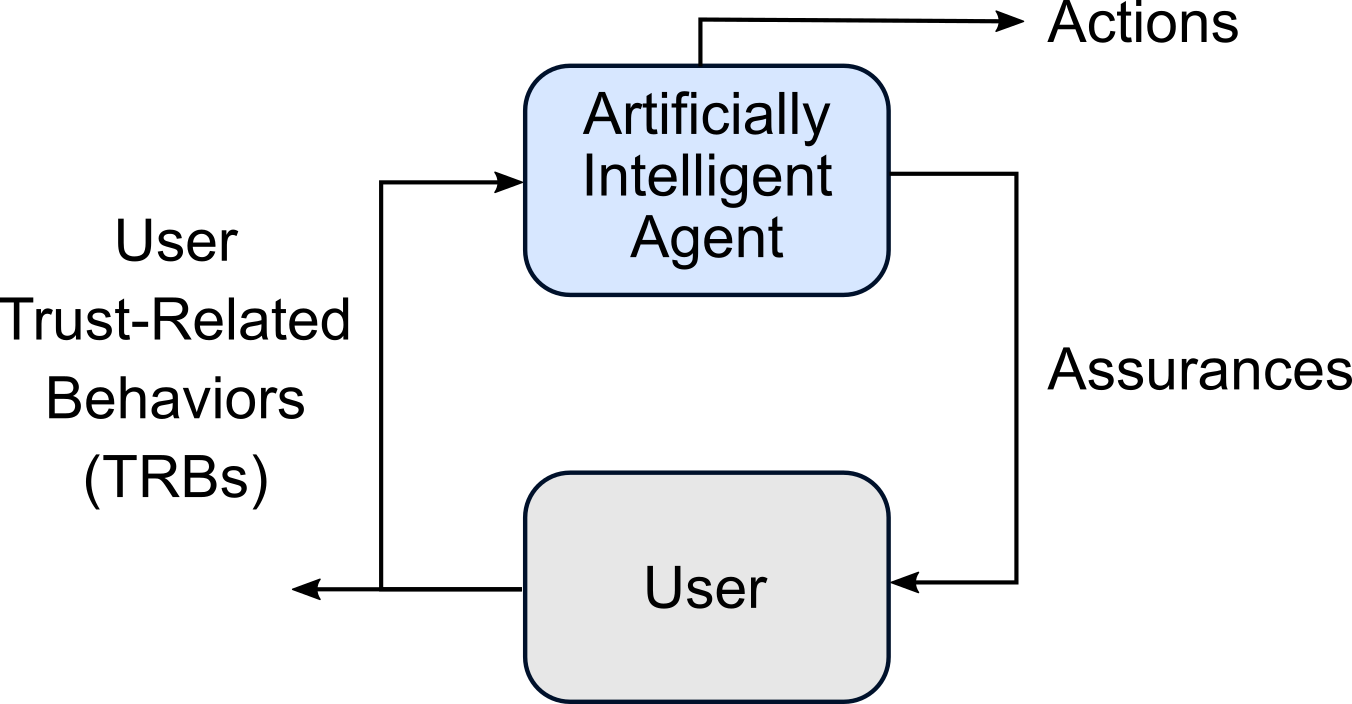
\includegraphics[width=0.5\textwidth]{Figures/SimpleTrust_one_way.png}
        \caption{stuff}
    \end{figure}

\section{Who cares?}
    Because everyone wants to trust their AIs, whether that be a single classification or regression algorithm, or a more interactive personal assistant that can understand language and communicate. Everyone wants to know how to trust these systems.  

    \paragraph{Why lay out AGI, when it doesn't exist yet?} Because this architecture is supposed to illustrate how the entire spectrum of AI from a single ML algorithm to an autonomous vehicle, to a full AGI operate on very similar grounds. That is that 

	\begin{sidewaysfigure}[htbp]
        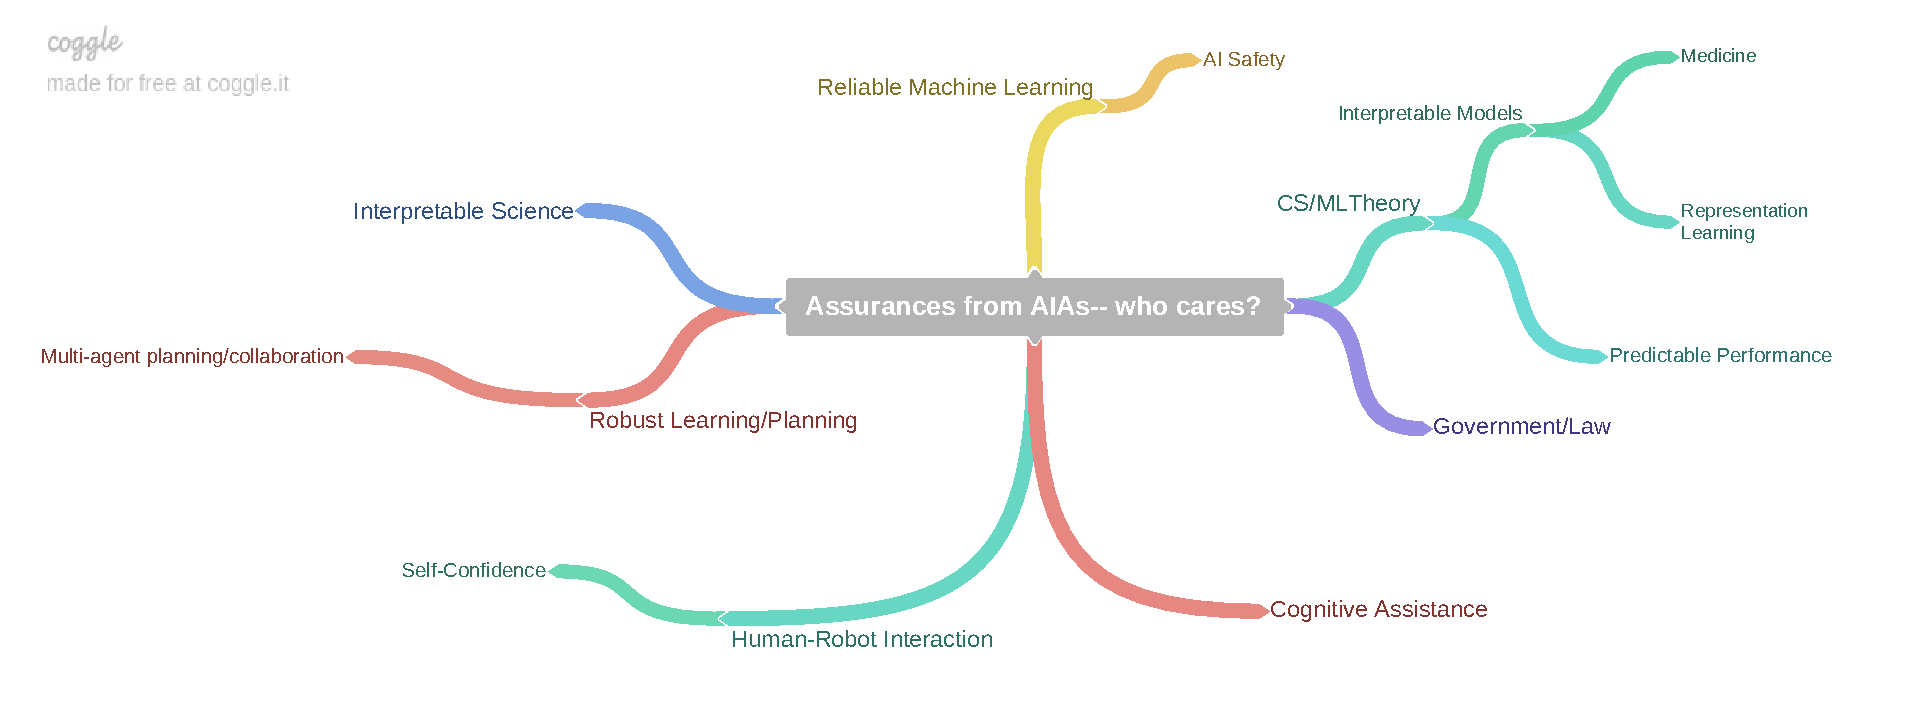
\includegraphics[width=8in]{Figures/WhoCares.pdf}%
    	\caption{A diagram showing some of the academic disciplines that want to trust AIs more fully}
        \label{fig:WhoCares}
    \end{sidewaysfigure}

    \paragraph{Science} Talk about why the science discplines care
    \paragraph{Robust Learning/Planning}
    \paragraph{HRI}
    \paragraph{Cognitive Assistance} 
    \paragraph{Government/Law} Regulations on the interpretability of certain algorithms, usage for assistants to lawyers.

    \textbf{Perhaps a table showing the field vs. the AI capability?}, this would help to illustrate the varying needs by fields. Perhaps highlight oversights?

